\iftoggle{arxiv}{
  \begin{figure}[!t]
  \begin{center}
    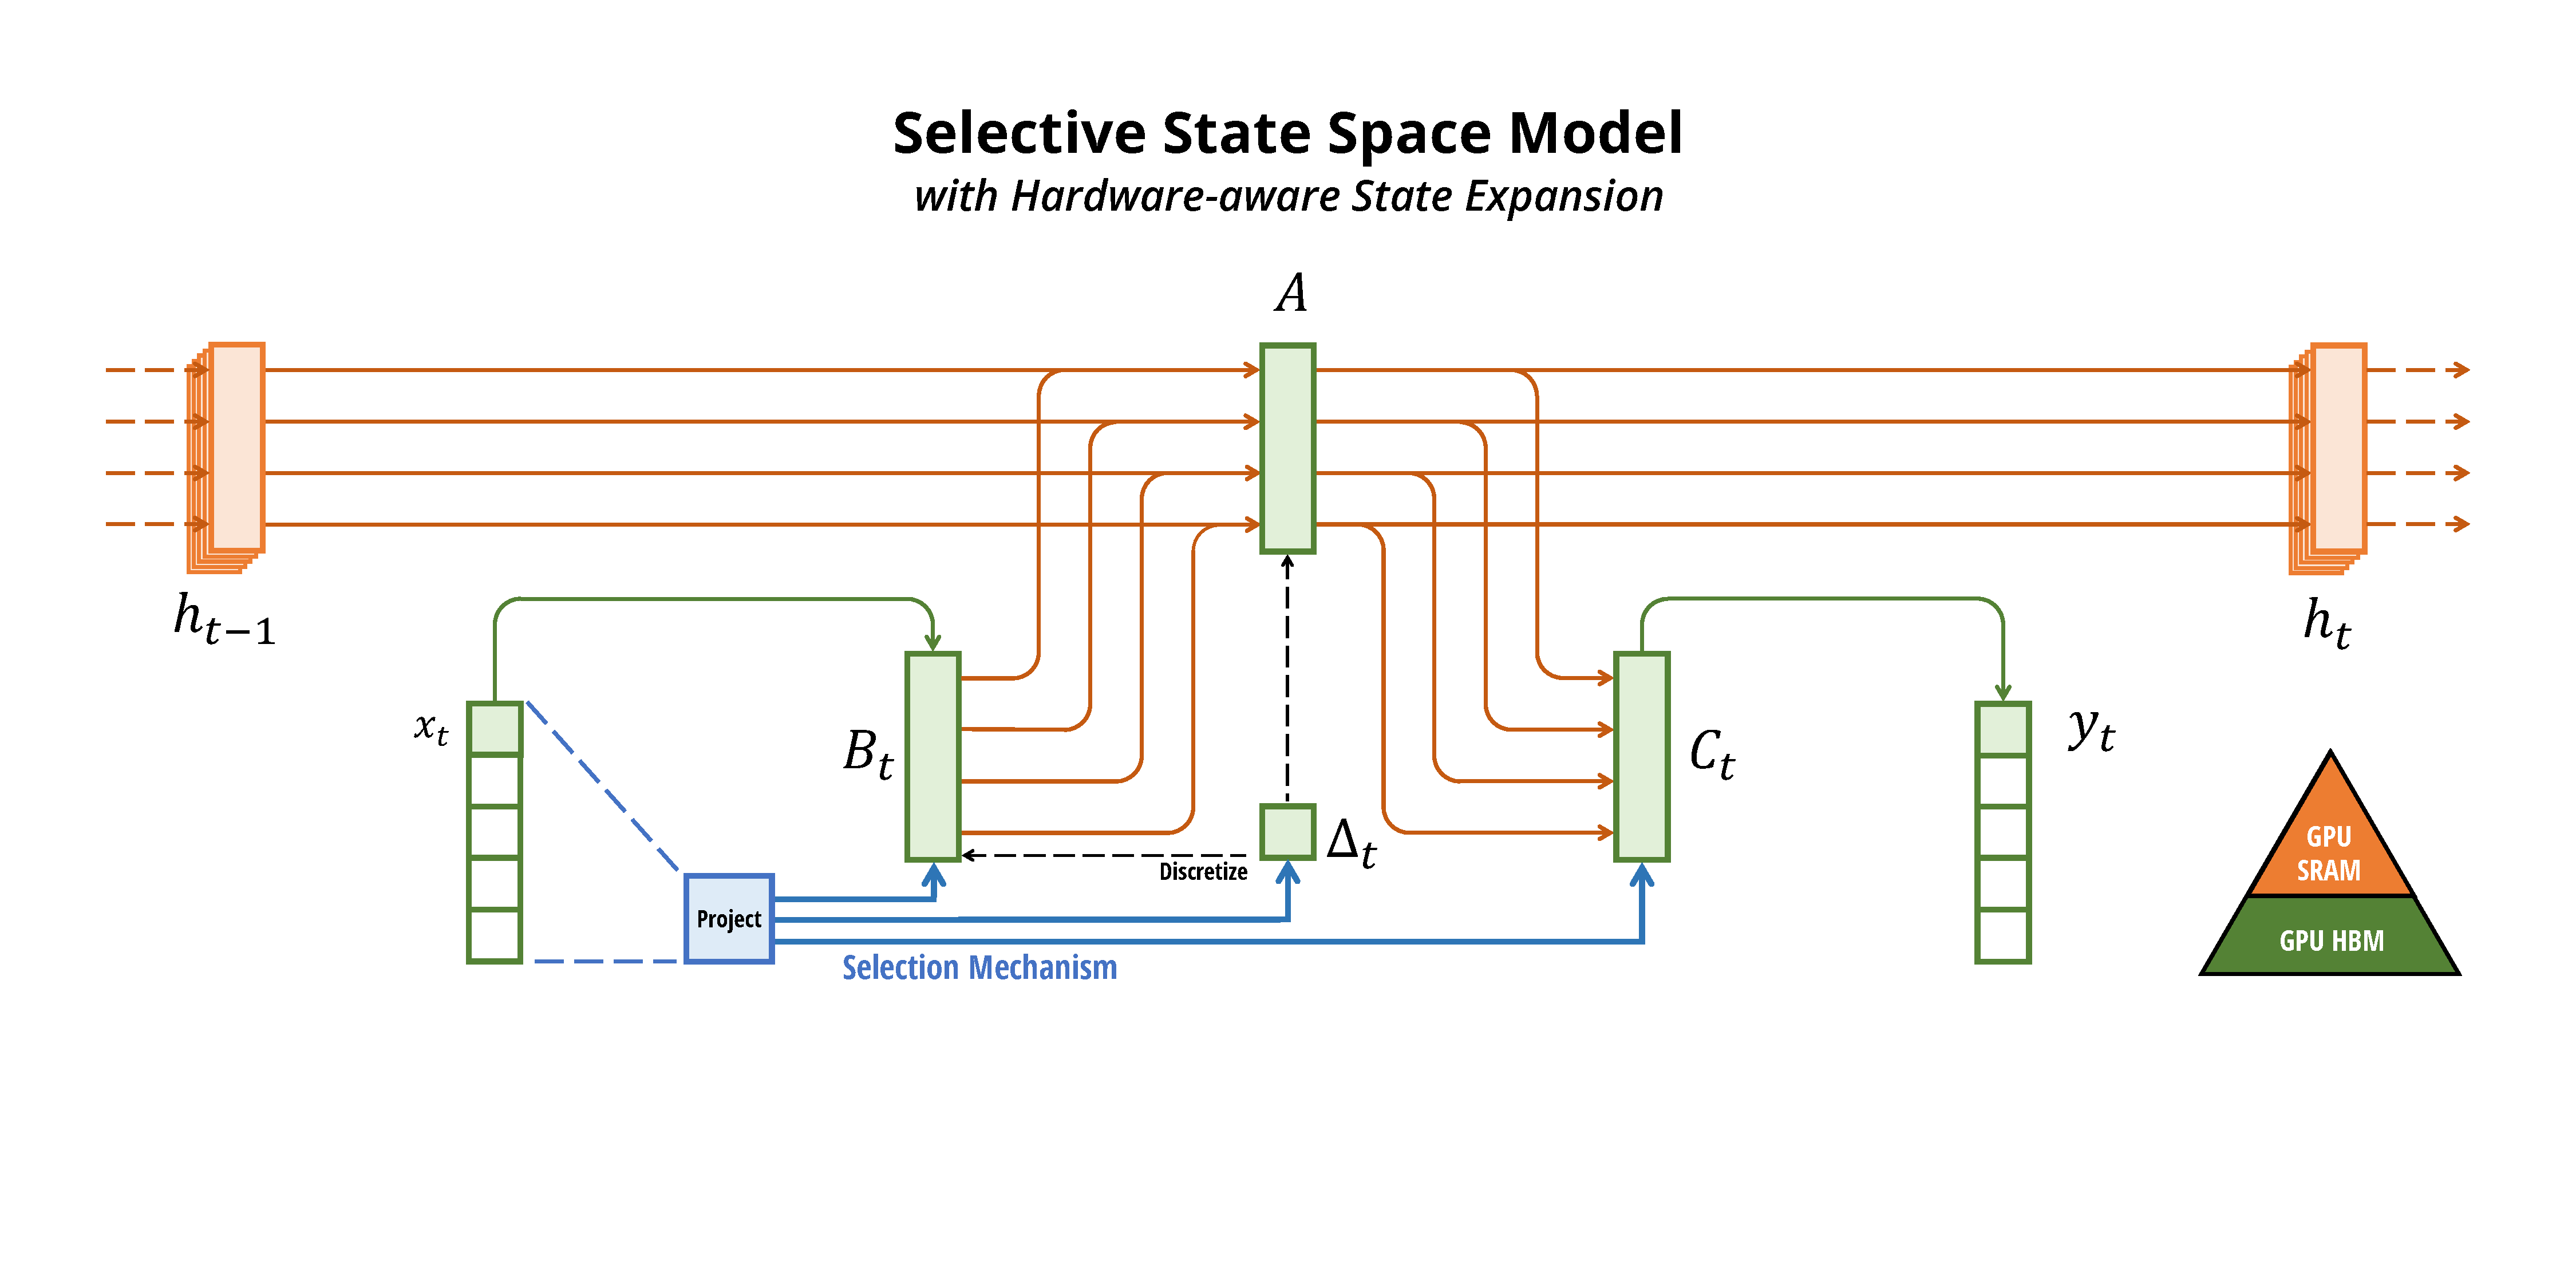
\includegraphics[width=\linewidth]{fig/selection.pdf}
  \end{center}
  \caption{
  (\textbf{Overview}.)
  Structured SSMs independently map each channel (e.g. $D=5$) of an input $x$ to output $y$ through a higher dimensional latent state $h$ (e.g.\ $N=4$).
  Prior SSMs avoid materializing this large effective state ($DN$, times batch size $B$ and sequence length $L$) through clever alternate computation paths requiring
  time-invariance: the $(\dt, \A, \B, \C)$ parameters are constant across time.
  Our selection mechanism adds back input-dependent dynamics, which
  also requires a careful hardware-aware algorithm to only materialize the expanded states in more efficient levels of the GPU memory hierarchy.
}
  \label{fig:selection}
\end{figure}
}{}


\section{State Space Models}
\label{sec:background}



Structured state space sequence models (S4) are a recent class of sequence models for deep learning that are broadly related to RNNs, and CNNs,
and classical state space models.
They are inspired by a particular continuous system \eqref{eq:ssm}
that maps a 1-dimensional function or sequence $x(t) \in \R \mapsto y(t) \in \R$ through an implicit latent state \( h(t) \in \R^N \). %
\iftoggle{arxiv}{

}{}
Concretely,
S4 models are defined with four parameters $(\dt, \A, \B, \C)$, which define a sequence-to-sequence transformation in two stages.

\begin{minipage}[t]{.30\linewidth}
  \begin{subequations}
    \label{eq:ssm}
    \begin{align}
      h'(t) &= \A h(t) + \B x(t) \\
      y(t) &= \C h(t)
    \end{align}
  \end{subequations}
\end{minipage}%
\begin{minipage}[t]{.30\linewidth}
  \begin{subequations}
    \label{eq:ssm:recurrence}
    \begin{align}
    \label{eq:ssm:recurrence:1}
      h_{t} &= \dA h_{t-1} + \dB x_t \\
    \label{eq:ssm:recurrence:2}
      y_t &= \C h_t
    \end{align}
  \end{subequations}
\end{minipage}%
\begin{minipage}[t]{.39\linewidth}
  \begin{subequations}%
    \label{eq:ssm:convolution}
    \begin{align}
      \label{eq:ssm:convolution:1}
      \bm{\overline{K}} &= (\bm{C}\bm{\overline{B}}, \bm{C}\bm{\overline{A}}\bm{\overline{B}}, \dots, \bm{C}\bm{\overline{A}}^{k}\bm{\overline{B}}, \dots) \\
      \label{eq:ssm:convolution:2}
      y &= x \ast \bm{\overline{K}}
    \end{align}
  \end{subequations}
\end{minipage}

\para{Discretization.}
The first stage transforms the ``continuous parameters'' $\dtAB$ to ``discrete parameters'' $\dAB$ through fixed formulas $\dA = f_A(\dt, \A)$ and $\dB = f_B(\dt, \A, \B)$,
where the pair $(f_A, f_B)$ is called a \emph{discretization rule}.
\iftoggle{arxiv}{
  Various rules can be used such as the zero-order hold (ZOH) defined in equation \eqref{eq:zoh}.
  \begin{equation}
    \label{eq:zoh}
    \dA = \exp(\dt \bm{A})
    \qquad
    \dB = (\dt \bm{A})^{-1} (\exp(\dt \bm{A}) - \bm{I}) \cdot \dt \bm{B}
  \end{equation}
}{
  The most common is zero-order hold (ZOH) defined by
  $\dA = \exp(\dt \bm{A})$
  and $\dB = (\dt \bm{A})^{-1} (\exp(\dt \bm{A}) - \bm{I}) \cdot \dt \bm{B}$.
}

Discretization has deep connections to continuous-time systems which can endow them with additional properties such as resolution invariance \citep{nguyen2022s4nd} and automatically ensuring that the model is properly normalized \citep{gu2023train,orvieto2023resurrecting}.
It also has connections to gating mechanisms of RNNs \citep{tallec2018can,gu2020improving} which we will revisit in \cref{sec:method:properties}.
However, from a mechanical point of view discretization can simply be viewed as the first step of the computation graph in the forward pass of an SSM.
\iftoggle{arxiv}{
  Alternate flavors of SSMs can bypass the discretization step and parameterize $\dAB$ directly instead~\citep{zhang2023effectively}, which may be easier to reason about.
}{}


\para{Computation.}
After the parameters have been transformed from $(\dt, \A, \B, \C) \mapsto (\dA, \dB, \C)$,
the model can be computed in two ways, either as a \textbf{linear recurrence} \eqref{eq:ssm:recurrence} or a \textbf{global convolution} \eqref{eq:ssm:convolution}.

Commonly, the model uses the convolutional mode \eqref{eq:ssm:convolution} for efficient parallelizable training (where the whole input sequence is seen ahead of time), %
and switched into recurrent mode \eqref{eq:ssm:recurrence} for efficient autoregressive inference (where the inputs are seen one timestep at a time).


\para{Linear Time Invariance (LTI).}
An important property of equations \eqref{eq:ssm} to \eqref{eq:ssm:convolution} is that the model's dynamics are constant through time.
In other words $\dtABC$, and consequently $\dAB$ as well, are fixed for all time-steps.
This property is called \emph{linear time invariance (LTI)}, which is deeply connected to recurrence and convolutions.
Informally, we think of LTI SSMs as being equivalent to any linear recurrence \eqref{eq:ssm:recurrence:1} or convolution \eqref{eq:ssm:convolution:2},
and use LTI as an umbrella term for these classes of models.

Thus far, all structured SSMs have been LTI (e.g.\ computed as convolutions) because of fundamental efficiency constraints, discussed in \cref{sec:method:scan}.
However, a core insight of this work is that LTI models have fundamental limitations in modeling certain types of data,
and our technical contributions involve removing the LTI constraint while overcoming the efficiency bottlenecks.


\para{Structure and Dimensions.}
Finally, we note that structured SSMs are so named because computing them efficiently also requires imposing structure on the $\A$ matrix.
The most popular form of structure is diagonal \citep{gupta2022diagonal,gu2022parameterization,smith2023s5}, which we also use.

In this case, the $\A \in \R^{N \times N}, \B \in \R^{N \times 1}, \C \in \R^{1 \times N}$ matrices can all be represented by $N$ numbers.
To operate over an input sequence $x$ of batch size $B$ and length $L$ with $D$ channels,
the SSM is applied independently to each channel.
Note that in this case, the total hidden state has dimension $DN$ per input, and computing it over the sequence length requires $O(BLDN)$ time and memory; this is the root of the fundamental efficiency bottleneck addressed in \cref{sec:method:scan}.

\iftoggle{arxiv}{
\para{General State Space Models.}
We note that the term \emph{state space model} has a very broad meaning which simply represents the notion of any recurrent process with a latent state.
It has been used to refer to many disparate concepts in different disciplines,
including Markov decision processes (MDP) (reinforcement learning~\citep{hafner2020dream}),
dynamic causal modeling (DCM) (computational neuroscience~\citep{friston2003dynamic}),
Kalman filters (controls~\citep{kalman1960new}),
hidden Markov models (HMM) and linear dynamical systems (LDS) (machine learning),
and recurrent (and sometimes convolutional) models at large (deep learning).


Throughout this entire paper we use the term ``SSM'' to refer exclusively to the class of structured SSMs or S4 models \citep{gu2022efficiently,gupta2022diagonal,gu2022parameterization,ma2023mega,smith2023s5,hasani2023liquid} and use these terms interchangeably.
For convenience we may also include derivatives of such models, such as those focusing on either the linear-recurrence or global-convolution viewpoints \citep{orvieto2023resurrecting,li2023makes,poli2023hyena}, and clarify nuances when necessary.
}{}

\para{SSM Architectures.}
SSMs are standalone sequence transformations that can be incorporated into end-to-end neural network architectures.
\iftoggle{arxiv}{
(We also sometimes call SSM architectures SSNNs, which are to SSM layers as CNNs are to linear convolution layers.)
}{}
We discuss some of the most well-known SSM architectures, many of which will also serve as our primary baselines.
\iftoggle{arxiv}{
\begin{itemize}[leftmargin=*]
}{
\begin{itemize}[leftmargin=*,itemsep=0pt,topsep=0pt]
}
  \item Linear attention~\citep{katharopoulos2020transformers} is an approximation of self-attention involving a recurrence which can be viewed as a degenerate linear SSM.
  \item H3~\citep{dao2023hungry} generalized this recurrence to use S4; it can be viewed as an architecture with an SSM sandwiched by two gated connections (\cref{fig:architecture}).
    H3 also inserts a standard local convolution, which they frame as a shift-SSM, before the main SSM layer.
  \item Hyena~\citep{poli2023hyena} uses the same architecture as H3 but replaces the S4 layer with an MLP-parameterized global convolution~\citep{romero2021ckconv}. %
    \iftoggle{arxiv}{
  \item RetNet~\citep{sun2023retentive} adds an additional gate to the architecture and uses a simpler SSM, allowing an alternative parallelizable computation path, using a variant of multi-head attention (MHA) instead of convolutions.
    \item RWKV~\citep{peng2023rwkv} is a recent RNN designed for language modeling based on another linear attention approximation, the attention-free Transformer~\citep{zhai2021attention}. Its main ``WKV'' mechanism involves LTI recurrences and can be viewed as the ratio of two SSMs.
    }{}
\end{itemize}
Other closely related SSMs and architectures are discussed further in an extended related work (\cref{sec:related}).
We highlight in particular S5~\citep{smith2023s5}, QRNN~\citep{bradbury2016quasi},
and SRU~\citep{lei2017simple},
which we view as the most closely related methods to our core selective SSM.

%



